\fontsize{13pt}{22.5pt}\selectfont

\section{CƠ SỞ LÝ THUYẾT}
\label{ch:theory}

\indent Chương này thiết lập nền tảng lý thuyết cho toàn bộ đồ án, đi từ bối cảnh lịch
sử của trí tuệ nhân tạo trong game tới bộ khái niệm hình thức của học tăng cường, rồi
tới năm thuật toán mà đề tài đem ra so sánh. Phần cuối chương dành cho Unity ML-Agents,
và dành nhiều nhất cho những giới hạn tích hợp của nền tảng này: chính các giới hạn ấy,
chứ không phải một lựa chọn học thuật nào, đã quy định cách đề tài phải bố trí thực
nghiệm ở Chương~\ref{ch:design}.

\subsection{Trí tuệ nhân tạo trong game}
\indent Trí tuệ nhân tạo trong game có lịch sử phát triển song hành với sự ra đời
của ngành công nghiệp game từ những thập niên 1970-1980. Khác với AI trong nghiên
cứu học thuật, AI trong game không nhất thiết phải tối ưu hay thông minh tuyệt đối
- mục tiêu cốt lõi là tạo ra những đối thủ hoặc nhân vật phi người chơi (NPC) có
hành vi đủ thuyết phục, góp phần mang lại trải nghiệm thú vị và thử thách cho người
chơi \cite{millington2019ai}. Theo thời gian, AI trong game đã trải qua hai giai đoạn
phát triển rõ rệt: từ các kỹ thuật lập trình hành vi cứng nhắc dựa trên quy tắc đến
các phương pháp học máy có khả năng thích nghi và tự cải thiện.

\subsubsection{AI truyền thống}
\indent Trong giai đoạn đầu, AI game chủ yếu dựa trên các hệ thống quy tắc cứng
(rule-based systems), trong đó lập trình viên định nghĩa trước toàn bộ hành vi của
NPC dưới dạng tập hợp các điều kiện và phản ứng tương ứng. Cách tiếp cận này dễ
kiểm soát và dự đoán được, nhưng thiếu tính linh hoạt khi gặp các tình huống ngoài
dự kiến.

\indent Để khắc phục hạn chế đó, máy trạng thái hữu hạn (Finite State Machine -
FSM) được ứng dụng rộng rãi trong những thập niên 1990-2000. FSM mô hình hóa hành
vi của NPC thông qua một tập hữu hạn các trạng thái (tuần tra, truy đuổi, tấn công,
rút lui) và các điều kiện chuyển trạng thái tương ứng. Nhờ tính đơn giản và hiệu quả
tính toán cao, FSM vẫn được sử dụng phổ biến trong nhiều thể loại game đến tận ngày
nay \cite{millington2019ai}. Tuy nhiên, khi số lượng trạng thái và điều kiện chuyển
tiếp tăng lên, FSM nhanh chóng trở nên phức tạp và khó bảo trì, dẫn đến hiện tượng
thường được gọi là ``state explosion''.

\indent Để giải quyết bài toán lập kế hoạch hành động phức tạp hơn, Goal-Oriented
Action Planning (GOAP) được giới thiệu và phổ biến qua tựa game F.E.A.R.
(2005) \cite{millington2019ai}. Thay vì định nghĩa cứng các chuyển trạng thái, GOAP
cho phép NPC tự lập kế hoạch hành động dựa trên mục tiêu hiện tại và trạng thái thế
giới, mang lại hành vi linh hoạt và tự nhiên hơn đáng kể. Dù vậy, toàn bộ tri thức
trong GOAP vẫn phải được lập trình thủ công bởi con người, khiến chi phí xây dựng
và mở rộng hệ thống tăng cao khi độ phức tạp của game tăng lên.

\subsubsection{AI học máy}
\indent Sự bùng nổ của học máy trong thập niên 2010 đã mở ra một
hướng tiếp cận hoàn toàn mới cho AI trong game. Thay vì lập trình hành vi thủ công,
các kỹ thuật học máy cho phép agent tự học từ dữ liệu hoặc từ tương tác với môi
trường. Trong số các hướng tiếp cận đó, học tăng cường (Reinforcement Learning -
RL) nổi lên như phương pháp phù hợp nhất với bản chất của game: agent học cách hành
động thông qua thử và sai, nhận phần thưởng hoặc hình phạt từ môi trường, và dần dần
tối ưu hóa chiến lược của mình để đạt điểm số cao nhất \cite{sutton2018reinforcement}.

\indent Bước ngoặt quan trọng đến vào năm 2013 khi DeepMind công bố thuật toán
DQN (Deep Q-Network) \cite{mnih2015humanlevel}, lần đầu tiên chứng minh một agent RL
có thể học chơi thành thạo 49 trò chơi Atari khác nhau chỉ từ dữ liệu pixel thô mà
không cần bất kỳ tri thức nào được lập trình sẵn. Thành tựu này đánh dấu sự ra đời
của Deep Reinforcement Learning - kết hợp sức mạnh biểu diễn của mạng nơ-ron sâu
với khả năng học từ tương tác của RL.

\indent Những năm tiếp theo chứng kiến hàng loạt thành tựu ấn tượng: AlphaGo và
AlphaGo Zero \cite{silver2016mastering, silver2017mastering} chinh phục cờ vây ở
trình độ kiện tướng thế giới; OpenAI Five \cite{openai2019dota} đánh bại các đội
chuyên nghiệp trong Dota~2; AlphaStar \cite{vinyals2019grandmaster} đạt danh hiệu
Grandmaster trong StarCraft~II. Các kết quả này vừa có giá trị học thuật, vừa
mở ra tiềm năng ứng dụng RL trực tiếp trong phát triển game thương mại, từ việc
tạo NPC thông minh đến sinh nội dung tự động và hỗ trợ kiểm thử game \cite{yannakakis2018artificial}.

\subsection{Nền tảng Reinforcement Learning}

\indent Học tăng cường (Reinforcement Learning - RL) là một nhánh của học máy trong
đó một tác nhân hay còn gọi là agent học cách hành động thông qua tương tác trực tiếp với môi
trường. Khác với học có giám sát, RL không yêu cầu dữ liệu gán nhãn
sẵn có; thay vào đó, agent tự khám phá không gian hành động và nhận phản hồi dưới
dạng phần thưởng hoặc hình phạt để dần dần cải thiện chiến lược của mình
\cite{sutton2018reinforcement}. Đây là đặc tính cốt lõi khiến RL trở nên phù hợp
với các bài toán game, nơi hành vi tối ưu thường khó định nghĩa tường minh nhưng lại
dễ đánh giá thông qua kết quả.

\subsubsection{Các khái niệm cơ bản}

\indent Vòng lặp tương tác trong RL được xây dựng xung quanh năm khái niệm nền tảng.
Agent là thực thể ra quyết định - trong bối cảnh game, agent có thể là
nhân vật người chơi, NPC hay robot mô phỏng. 

\indent Environment hay môi trường là thế giới mà agent tương tác, bao gồm toàn bộ các đối tượng, luật chơi và cơ chế phản hồi; trong đề tài này, môi trường là các scene 3D được xây dựng trong Unity.

\indent State hay trạng thái $s \in \mathcal{S}$ là biểu diễn của môi trường
tại một thời điểm nhất định mà agent có thể quan sát được. Trong môi trường 3D, state
thường bao gồm vị trí, vận tốc của các đối tượng, khoảng cách đến mục tiêu và các
thông tin không gian liên quan. Action hay hành động $a \in \mathcal{A}$ là
tập hợp các lựa chọn mà agent có thể thực hiện tại mỗi bước, có thể là rời rạc như di chuyển lên,xuống,trái,phải hoặc liên tục như lực đẩy
theo trục $x$, $y$, $z$.

\indent Reward hay phần thưởng $r_t \in \mathbb{R}$ là tín hiệu phản hồi mà
môi trường trả về sau mỗi hành động của agent, đóng vai trò là thước đo duy nhất để
agent đánh giá chất lượng quyết định của mình. Việc thiết kế hàm phần thưởng hợp lý
là một trong những bước quan trọng và khó nhất trong quá trình xây dựng hệ thống RL,
vì một hàm phần thưởng không phù hợp có thể dẫn đến hành vi không mong muốn dù thuật
toán hoạt động đúng về mặt lý thuyết \cite{sutton2018reinforcement}.

\indent Tại mỗi bước thời gian $t$, agent quan sát trạng thái $s_t$, thực hiện hành
động $a_t$, nhận phần thưởng $r_t$ và chuyển sang trạng thái mới $s_{t+1}$. Vòng lặp
này lặp lại liên tục cho đến khi episode kết thúc, tức khi agent hoàn thành nhiệm vụ,
thất bại hoặc vượt quá số bước tối đa, và hình thành nên một quỹ đạo tương tác
$\tau = (s_0, a_0, r_0, s_1, a_1, r_1, \ldots)$. Toàn bộ vòng lặp tương tác giữa agent
và môi trường được minh họa trong Hình~\ref{fig:rl_loop}. Đây là sơ đồ khái quát nhất
của mọi hệ thống học tăng cường: agent quan sát trạng thái hiện tại của môi trường,
lựa chọn một hành động dựa trên chính sách của mình, và môi trường phản hồi lại bằng
một trạng thái mới cùng một phần thưởng, cứ thế lặp đi lặp lại để agent dần cải thiện
chính sách.

\begin{figure}[H]
    \centering
    \begin{tikzpicture}[node distance=2.2cm, >=latex]
        \node[draw, rounded corners, minimum width=3cm, minimum height=1.1cm,
              fill=ppocolor!15] (agent) at (0,1.6) {Agent (Tác nhân)};
        \node[draw, rounded corners, minimum width=3cm, minimum height=1.1cm,
              fill=saccolor!15] (env) at (0,-1.6) {Environment (Môi trường)};
        \draw[->, thick] (agent.east) .. controls (4.2,1.6) and (4.2,-1.6) ..
              node[right, align=left, font=\small] {Hành động $a_t$} (env.east);
        \draw[->, thick] (env.west) .. controls (-4.2,-1.6) and (-4.2,1.6) ..
              node[left, align=right, font=\small]
              {Trạng thái $s_{t+1}$\\ Phần thưởng $r_{t+1}$} (agent.west);
    \end{tikzpicture}
    \caption{Vòng lặp tương tác giữa agent và môi trường trong học tăng cường}
    \label{fig:rl_loop}
\end{figure}

\subsubsection{Markov Decision Process}
\label{sub:mdp}

\indent Hầu hết các bài toán RL được hình thức hóa dưới dạng Quá trình Quyết định
Markov (Markov Decision Process - MDP), một khung toán học cung cấp nền tảng lý
thuyết chặt chẽ cho việc mô hình hóa bài toán ra quyết định tuần tự trong môi trường
ngẫu nhiên \cite{puterman1994markov}. Một MDP được định nghĩa bởi bộ năm thành phần
$\mathcal{M} = (\mathcal{S}, \mathcal{A}, \mathcal{P}, \mathcal{R}, \gamma)$, trong
đó $\mathcal{S}$ là không gian trạng thái, $\mathcal{A}$ là không gian hành động,
$\mathcal{P}$ là hàm chuyển trạng thái, $\mathcal{R}$ là hàm phần thưởng và $\gamma
\in [0, 1)$ là hệ số chiết khấu.

\indent Hàm chuyển trạng thái $\mathcal{P}(s' \mid s, a)$ xác định xác suất chuyển
từ trạng thái $s$ sang trạng thái $s'$ khi thực hiện hành động $a$. Tính chất Markov
- hay còn gọi là tính không nhớ - đòi hỏi rằng trạng thái tiếp theo $s_{t+1}$
chỉ phụ thuộc vào trạng thái hiện tại $s_t$ và hành động $a_t$, không phụ thuộc vào
lịch sử trước đó:

\begin{equation}
    \mathcal{P}(s_{t+1} \mid s_t, a_t, s_{t-1}, a_{t-1}, \ldots) =
    \mathcal{P}(s_{t+1} \mid s_t, a_t)
\end{equation}

\indent Giả thiết Markov là thứ giữ cho bài toán còn giải được: nhờ nó, agent chỉ cần
quan sát trạng thái hiện tại để ra quyết định tối ưu thay vì phải lưu trữ và xử lý toàn
bộ lịch sử tương tác. Trong thực tế, nhiều môi trường game thỏa mãn gần đúng tính chất này nếu
state được thiết kế đủ phong phú để mang đầy đủ thông tin cần thiết.

\indent Hệ số chiết khấu $\gamma$ xác định mức độ agent coi trọng phần thưởng tương
lai so với phần thưởng hiện tại. Khi $\gamma$ gần 1, agent có xu hướng lập kế hoạch
dài hạn; khi $\gamma$ nhỏ, agent tập trung vào phần thưởng tức thời. Tổng phần thưởng
tích lũy có chiết khấu mà agent hướng đến tối đa hóa được định nghĩa là:

\begin{equation}
    G_t = \sum_{k=0}^{\infty} \gamma^k r_{t+k+1}
\end{equation}

\subsubsection{Policy và Value Function}

\indent Policy (chính sách) $\pi$ là hàm ánh xạ từ trạng thái sang hành
động, định nghĩa chiến lược hành động của agent. Policy có thể là tất định
$\pi: \mathcal{S} \rightarrow \mathcal{A}$ hoặc ngẫu nhiên $\pi(a \mid s) =
P(A_t = a \mid S_t = s)$, cho biết xác suất chọn hành động $a$ khi ở trạng thái $s$.
Mục tiêu của RL là tìm policy tối ưu $\pi^*$ sao cho tổng phần thưởng tích lũy kỳ
vọng là lớn nhất.

\indent Value Function hay còn được gọi là hàm giá trị đo lường mức độ tốt của một trạng thái
hoặc một cặp trạng thái-hành động khi agent tuân theo một policy nhất định. Hàm giá
trị trạng thái $V^\pi(s)$ được định nghĩa là tổng phần thưởng tích lũy kỳ vọng khi
bắt đầu từ trạng thái $s$ và tuân theo policy $\pi$:

\begin{equation}
    V^\pi(s) = \mathbb{E}_\pi \left[ G_t \mid S_t = s \right]
             = \mathbb{E}_\pi \left[ \sum_{k=0}^{\infty} \gamma^k r_{t+k+1}
               \mid S_t = s \right]
\end{equation}

\indent Hàm giá trị hành động $Q^\pi(s, a)$ (hay Q-function) mở rộng khái niệm trên
bằng cách đánh giá giá trị của việc thực hiện hành động $a$ tại trạng thái $s$ rồi
sau đó tuân theo policy $\pi$:

\begin{equation}
    Q^\pi(s, a) = \mathbb{E}_\pi \left[ G_t \mid S_t = s, A_t = a \right]
\end{equation}

\indent Mối quan hệ giữa $V^\pi$ và $Q^\pi$ được thể hiện qua phương trình Bellman
\cite{bellman1957markovian}, nền tảng lý thuyết của hầu hết các thuật toán RL hiện
đại:

\begin{equation}
    V^\pi(s) = \sum_{a} \pi(a \mid s) \, Q^\pi(s, a)
\end{equation}

\indent Policy tối ưu $\pi^*$ và hàm giá trị tối ưu $V^*(s)$, $Q^*(s,a)$ thỏa mãn
phương trình tối ưu Bellman:

\begin{equation}
    Q^*(s, a) = \mathbb{E} \left[ r_{t+1} + \gamma \max_{a'} Q^*(s_{t+1}, a')
                \mid S_t = s, A_t = a \right]
\end{equation}

\indent Trong thực tế, với không gian trạng thái lớn và liên tục như các môi trường
game 3D, việc biểu diễn chính xác $V^\pi$ hay $Q^\pi$ dưới dạng bảng tra cứu là
không khả thi. Đây là động lực dẫn đến sự ra đời của Deep Reinforcement Learning,
trong đó các hàm giá trị và policy được xấp xỉ bằng mạng nơ-ron sâu, được trình bày
chi tiết trong Mục~\ref{sub:deeprl}.

\subsection{Học tăng cường sâu}
\label{sub:deeprl}
\indent Học tăng cường sâu (Deep Reinforcement Learning) là sự kết hợp giữa học tăng cường và
mạng nơ-ron sâu (deep neural network), ra đời nhằm giải quyết hạn chế cốt lõi của RL
truyền thống khi đối mặt với các bài toán có không gian trạng thái và hành động lớn,
liên tục. Thay vì lưu trữ giá trị của từng cặp trạng thái-hành động trong bảng tra
cứu, Deep RL sử dụng mạng nơ-ron để xấp xỉ các hàm giá trị hoặc policy, cho phép
tổng quát hóa sang các trạng thái chưa từng gặp trong quá trình huấn luyện
\cite{lecun2015deep}. Đây là đặc tính then chốt khiến Deep RL có thể xử lý được các
môi trường game 3D phức tạp như trong đề tài này.

\subsubsection{Vai trò của mạng Neural Network trong RL}
\indent Trong RL truyền thống, hàm giá trị $Q(s, a)$ hoặc policy $\pi(a \mid s)$
được biểu diễn dưới dạng bảng tra cứu (lookup table), đòi hỏi mỗi cặp $(s, a)$ phải
được thăm viếng đủ nhiều lần để ước lượng chính xác. Cách tiếp cận này chỉ khả thi
với không gian trạng thái hữu hạn và nhỏ. Với các môi trường game 3D, không gian
trạng thái có thể là liên tục và có số chiều rất lớn - ví dụ, vector quan sát của
agent trong môi trường Football Table bao gồm vị trí, vận tốc của bóng và các thanh
gạt trong không gian ba chiều - khiến bảng tra cứu hoàn toàn không khả thi.

\indent Mạng nơ-ron sâu giải quyết vấn đề này bằng cách đóng vai trò là bộ xấp xỉ
hàm tổng quát (universal function approximator). Thay vì lưu trữ giá trị cho từng
trạng thái, mạng học một ánh xạ tham số hóa $f_\theta: \mathcal{S} \rightarrow
\mathbb{R}$ (đối với value function) hoặc $f_\theta: \mathcal{S} \rightarrow
\Delta(\mathcal{A})$ (đối với policy), trong đó $\theta$ là tập tham số của mạng được
tối ưu hóa qua quá trình huấn luyện. Nhờ khả năng tổng quát hóa, mạng có thể ước
lượng giá trị hoặc đưa ra hành động cho các trạng thái chưa từng gặp dựa trên sự
tương đồng với các trạng thái đã học \cite{sutton2018reinforcement}.

\indent Trong thực tế, kiến trúc mạng được lựa chọn tùy theo dạng dữ liệu quan sát.
Với dữ liệu dạng vector số thực (vị trí, vận tốc, khoảng cách), mạng fully-connected
nhiều lớp (MLP) là lựa chọn phổ biến và hiệu quả. Với dữ liệu dạng ảnh hoặc dữ liệu
không gian, mạng tích chập (CNN) thường được ưu tiên. Unity ML-Agents hỗ trợ cả hai
kiến trúc này và cho phép tùy chỉnh số lớp ẩn cũng như số đơn vị trong mỗi lớp thông
qua tệp cấu hình YAML.

\subsubsection{Phân loại: Policy-Based, Value-Based, Actor-Critic}
\indent Các thuật toán Deep RL hiện đại được phân loại thành ba nhóm chính dựa trên
đối tượng mà mạng nơ-ron học để xấp xỉ, mỗi nhóm có ưu nhược điểm riêng và phù hợp
với các dạng bài toán khác nhau.

\indent Value-Based là nhóm thuật toán trong đó mạng nơ-ron học xấp xỉ hàm
giá trị $Q(s, a)$, từ đó suy ra policy tối ưu bằng cách chọn hành động có giá trị
$Q$ cao nhất. Đại diện tiêu biểu là DQN \cite{mnih2015humanlevel}. Nhóm này hoạt
động tốt với không gian hành động rời rạc nhưng gặp khó khăn với không gian hành động
liên tục do không thể tối ưu $\max_a Q(s,a)$ một cách hiệu quả khi $\mathcal{A}$ là
liên tục.

\indent Policy-Based là nhóm thuật toán trực tiếp tham số hóa và tối ưu
policy $\pi_\theta(a \mid s)$ bằng cách tính gradient của hàm mục tiêu theo tham số
$\theta$ thông qua phương pháp policy gradient \cite{williams1992simple}. Nhóm này xử
lý tốt cả không gian hành động rời rạc lẫn liên tục, nhưng thường có phương sai cao
trong ước lượng gradient, dẫn đến quá trình huấn luyện kém ổn định. PPO
\cite{schulman2017proximal} thuộc nhóm này, bổ sung thêm cơ chế clipping để giới hạn
độ lớn của mỗi bước cập nhật, giúp ổn định quá trình huấn luyện đáng kể.

\indent Actor-Critic là nhóm kết hợp ưu điểm của cả hai nhóm trên bằng cách
duy trì đồng thời hai mạng nơ-ron: mạng actor học policy $\pi_\theta(a \mid
s)$ và mạng critic học hàm giá trị $V_\phi(s)$ hoặc $Q_\phi(s,a)$. Critic
đóng vai trò đánh giá chất lượng hành động của actor, cung cấp tín hiệu học ổn định
hơn so với việc chỉ dựa vào phần thưởng thực tế \cite{mnih2016asynchronous}. SAC
\cite{haarnoja2018soft} và MA-POCA \cite{cohen2022mapoca} đều thuộc nhóm Actor-Critic,
trong đó SAC bổ sung thêm entropy regularization để khuyến khích agent khám phá, còn
MA-POCA mở rộng kiến trúc critic sang bài toán đa tác nhân với cơ chế centralized
critic cho phép mỗi agent học dựa trên thông tin toàn cục trong quá trình huấn luyện.

\indent Bảng~\ref{tab:rl_comparison} tóm tắt vị trí của năm thuật toán được sử dụng
trong đề tài theo cách phân loại trên.

\begin{table}[H]
\centering
\caption{Phân loại các thuật toán sử dụng trong đề tài}
\label{tab:rl_comparison}
\renewcommand{\arraystretch}{1.4}
\tablefont
\begin{tabular}{|>{\centering\arraybackslash}p{2.5cm}
                |>{\centering\arraybackslash}p{3cm}
                |>{\centering\arraybackslash}p{3cm}
                |>{\centering\arraybackslash}p{4.5cm}|}
\hline
\textbf{Thuật toán} & \textbf{Nhóm} & \textbf{On/Off-policy} & \textbf{Phù hợp với} \\
\hline
PPO      & Policy-Based      & On-policy  & Đối kháng, điều hướng \\
\hline
SAC      & Actor-Critic      & Off-policy & Hành động liên tục    \\
\hline
MA-POCA  & Actor-Critic      & On-policy  & Hợp tác đa tác nhân   \\
\hline
MAPPO    & Policy-Based      & On-policy  & Hợp tác, tác nhân đồng nhất \\
\hline
DQN      & Value-Based       & Off-policy & Hành động rời rạc \\
\hline
\end{tabular}
\end{table}

\subsubsection{Phần thưởng tò mò nội tại}
\label{sub:curiosity}

\indent Trong các bài toán học tăng cường thực tế, đặc biệt là các môi trường game 3D phức tạp như Capture The Flag hay Cross The Road, tín hiệu phần thưởng ngoại sinh thường rất thưa thớt hoặc bị trì hoãn. Nếu tác nhân chỉ dựa vào phần thưởng từ môi trường để học, nó có thể dành phần lớn thời gian đầu khám phá ngẫu nhiên mà không nhận được bất kỳ tín hiệu hữu ích nào, dẫn đến việc không thể học được chính sách hiệu quả. Để giải quyết vấn đề này, cơ chế phần thưởng tò mò nội tại (Intrinsic Curiosity) đã được đề xuất nhằm khuyến khích tác nhân chủ động khám phá những trạng thái mới mẻ của môi trường.

\indent Trong đồ án này, cơ chế tò mò được tích hợp thông qua mô hình Intrinsic Curiosity Module (ICM) do Pathak và cộng sự \cite{pathak2017curiosity} đề xuất. Ý tưởng cốt lõi của ICM là sử dụng sai số dự đoán (prediction error) làm tín hiệu phần thưởng nội tại: tác nhân sẽ nhận được phần thưởng cao khi nó chuyển đến một trạng thái mà mô hình nội tại của nó không thể dự đoán chính xác.

\indent Kiến trúc của ICM bao gồm hai mạng nơ-ron con hoạt động song song: mô hình ngược (Inverse Model) và mô hình thuận (Forward Model). Để tránh việc tác nhân bị thu hút bởi những yếu tố ngẫu nhiên không thể dự đoán trong môi trường (hiện tượng tivi nhiễu hạt - noisy TV problem), ICM không dự đoán trực tiếp trạng thái thô $s_t$, mà dự đoán đặc trưng ẩn $\phi(s_t)$ được trích xuất qua một mạng mã hóa (Encoder).

\indent \textbf{Mô hình ngược (Inverse Model):} Mạng này nhận đầu vào là đặc trưng của trạng thái hiện tại $\phi(s_t)$ và đặc trưng của trạng thái tiếp theo $\phi(s_{t+1})$, sau đó dự đoán hành động $\hat{a}_t$ đã gây ra sự chuyển tiếp này. Hàm mất mát của Inverse Model được định nghĩa là:
\begin{equation}
    L_{\text{inv}} = \mathbb{E} \left[ -\log P(\hat{a}_t = a_t \mid \phi(s_t), \phi(s_{t+1})) \right]
\end{equation}
Việc huấn luyện Inverse Model buộc mạng mã hóa $\phi$ chỉ giữ lại những thông tin trạng thái có liên quan trực tiếp đến hành động của tác nhân, loại bỏ các chi tiết nhiễu vô ích.

\indent \textbf{Mô hình thuận (Forward Model):} Mạng này nhận đầu vào là đặc trưng trạng thái hiện tại $\phi(s_t)$ và hành động $a_t$, từ đó dự đoán đặc trưng của trạng thái tiếp theo $\hat{\phi}(s_{t+1})$. Hàm mất mát của Forward Model thường là sai số bình phương trung bình:
\begin{equation}
    L_{\text{fwd}} = \frac{1}{2} \left\| \hat{\phi}(s_{t+1}) - \phi(s_{t+1}) \right\|^2_2
\end{equation}

\indent \textbf{Phần thưởng tò mò:} Sai số của Forward Model chính là thước đo sự ``ngạc nhiên'' của tác nhân. Phần thưởng tò mò $r_t^i$ được định nghĩa tỷ lệ thuận với sai số này:
\begin{equation}
    r_t^i = \eta \frac{1}{2} \left\| \hat{\phi}(s_{t+1}) - \phi(s_{t+1}) \right\|^2_2
\end{equation}
\noindent trong đó $\eta$ là hệ số tỷ lệ. Tổng phần thưởng mà tác nhân nhận được tại mỗi bước sẽ là sự kết hợp có trọng số giữa phần thưởng ngoại sinh và phần thưởng nội tại: $r_t = r_t^e + \beta r_t^i$. Trong các thực nghiệm của đề tài, $\beta$ thường được đặt ở mức $0{,}02$ nhằm bảo đảm tác nhân vẫn hướng tới mục tiêu chính của trò chơi.

\begin{figure}[H]
    \centering
    \begin{tikzpicture}[>=stealth, 
        box/.style={rectangle, draw, thick, minimum width=2.5cm, minimum height=1cm, align=center},
        arrow/.style={->, thick}
    ]
        % State inputs
        \node (st) at (-3,4) {$s_t$};
        \node (st1) at (-3,0) {$s_{t+1}$};
        
        % Features
        \node (phi_st) [box] at (0,4) {Đặc trưng \\ $\phi(s_t)$};
        \node (phi_st1) [box] at (0,0) {Đặc trưng \\ $\phi(s_{t+1})$};
        
        % Action input
        \node (at) at (3.5, 6) {$a_t$};
        
        % Models
        \node (fwd) [box, fill=red!10] at (3.5,4) {Forward Model};
        \node (inv) [box, fill=blue!10] at (3.5,2) {Inverse Model};
        
        % Outputs
        \node (phi_hat) at (6.5,4) {$\hat{\phi}(s_{t+1})$};
        \node (ahat) at (6.5,2) {$\hat{a}_t$};
        \node (loss) [box, fill=green!10] at (6.5, 0) {Tính sai số \\ $r_t^i$};
        
        % Encoders
        \draw[arrow] (st) -- (phi_st) node[midway, above] {Encoder};
        \draw[arrow] (st1) -- (phi_st1) node[midway, above] {Encoder};
        
        % Forward model
        \draw[arrow] (phi_st) -- (fwd);
        \draw[arrow] (at) -- (fwd);
        \draw[arrow] (fwd) -- (phi_hat);
        
        % Inverse model (routing to avoid crossing)
        \draw[arrow, rounded corners] (phi_st.south) |- ([yshift=2mm]inv.west);
        \draw[arrow, rounded corners] (phi_st1.north) |- ([yshift=-2mm]inv.west);
        \draw[arrow] (inv) -- (ahat);
        
        % Loss calculation
        \draw[arrow] (phi_hat) -- (loss);
        \draw[arrow] (phi_st1) -- (loss);
        
    \end{tikzpicture}
    \caption{Sơ đồ kiến trúc Intrinsic Curiosity Module (ICM)}
    \label{fig:icm_arch}
\end{figure}

\subsection{Các thuật toán sử dụng trong đề tài}

\indent Đề tài sử dụng năm thuật toán học tăng cường đại diện cho các hướng tiếp cận
khác nhau: PPO thuộc nhóm policy-based on-policy đơn tác nhân, SAC thuộc nhóm
actor-critic off-policy, MA-POCA là thuật toán chuyên biệt cho bài toán đa tác nhân
dựa trên cơ chế attention, MAPPO là mở rộng của PPO cho đa tác nhân thông qua chia
sẻ tham số, và DQN đại diện cho nhóm phương pháp dựa trên giá trị. Phần này trình bày
nguyên lý hoạt động và đặc điểm của từng thuật toán,
làm cơ sở cho việc lựa chọn và phân tích kết quả thực nghiệm ở các chương sau.

\subsubsection{PPO}
\label{sub:ppo}
\indent PPO (Proximal Policy Optimization) được Schulman và cộng sự đề xuất vào năm
2017 \cite{schulman2017proximal} như một cải tiến của TRPO (Trust Region Policy
Optimization) \cite{schulman2015trust} nhằm giữ lại tính ổn định trong cập nhật
policy nhưng đơn giản hơn đáng kể về mặt triển khai. PPO hiện là một trong những
thuật toán RL phổ biến nhất trong cả nghiên cứu lẫn ứng dụng thực tế, và là thuật
toán on-policy mặc định trong Unity ML-Agents.

\indent Về nguyên lý hoạt động, PPO là thuật toán on-policy, nghĩa là dữ liệu
huấn luyện được thu thập trực tiếp từ policy hiện tại và bị loại bỏ sau mỗi lần cập
nhật. Ý tưởng cốt lõi của PPO là giới hạn độ lớn thay đổi của policy trong mỗi bước
cập nhật, tránh tình trạng policy thay đổi quá đột ngột dẫn đến suy giảm hiệu năng
không thể phục hồi - một vấn đề phổ biến trong các thuật toán policy gradient đơn
giản.

\indent PPO đạt được điều này thông qua hàm mục tiêu clipped surrogate:

\begin{equation}
    L^{\text{CLIP}}(\theta) = \mathbb{E}_t \left[
        \min \left(
            r_t(\theta) \hat{A}_t,\;
            \text{clip}\!\left(r_t(\theta),\, 1-\varepsilon,\, 1+\varepsilon\right)
            \hat{A}_t
        \right)
    \right]
\end{equation}

\noindent trong đó $r_t(\theta) = \dfrac{\pi_\theta(a_t \mid s_t)}{\pi_{\theta_\text{old}}(a_t \mid s_t)}$
là tỷ lệ xác suất giữa policy mới và policy cũ, $\hat{A}_t$ là ước lượng advantage
(mức độ hành động tốt hơn hoặc kém hơn kỳ vọng trung bình) và $\varepsilon$ là siêu
tham số clipping thường được đặt trong khoảng $[0.1, 0.2]$. Toán tử $\text{clip}$
giới hạn $r_t(\theta)$ trong khoảng $[1-\varepsilon, 1+\varepsilon]$, ngăn policy mới
lệch quá xa policy cũ trong một bước cập nhật. Hàm $\min$ đảm bảo mục tiêu luôn là
cận dưới thận trọng (pessimistic lower bound) của mục tiêu không clipped.

\indent Giá trị advantage $\hat{A}_t$ xuất hiện trong biểu thức trên thường được ước
lượng theo phương pháp Generalized Advantage Estimation (GAE), một cách dung hòa giữa
độ lệch và phương sai của ước lượng thông qua tham số $\lambda$:

\begin{equation}
    \hat{A}_t = \sum_{l=0}^{\infty} (\gamma\lambda)^l \delta_{t+l}, \quad
    \delta_t = r_t + \gamma V(s_{t+1}) - V(s_t)
\end{equation}

\noindent trong đó $\lambda \in [0,1]$ là tham số cân bằng giữa bias và phương sai
của ước lượng advantage, $V(s_t)$ là giá trị trạng thái được ước lượng bởi mạng
critic.

\indent Trong mỗi iteration, PPO thu thập một batch dữ liệu từ môi trường bằng policy
hiện tại, sau đó thực hiện nhiều lần cập nhật gradient trên cùng batch đó (thường từ
3 đến 10 epochs) trước khi thu thập batch mới. Nhờ cơ chế clipping, các lần cập nhật
lặp lại này không làm policy lệch quá xa điểm xuất phát, đảm bảo tính ổn định mà
không cần tính toán tốn kém như TRPO.

\indent \textbf{Ưu điểm:} Thế mạnh thật sự của PPO không nằm ở chất lượng chính sách
cuối cùng mà ở chỗ nó hiếm khi hỏng. Clipping chặn trên độ lớn của mỗi bước cập nhật,
nên một tốc độ học đặt sai thường chỉ làm chậm quá trình học chứ không phá sập chính
sách như ở các phương pháp policy gradient thuần túy. Thuật toán chạy được trên cả không
gian hành động rời rạc lẫn liên tục và đi kèm sẵn cơ chế self-play trong ML-Agents. Vì
đặc tính bền này, đề tài chọn PPO làm mốc so sánh: mọi thuật toán khác đều được đối chiếu
với nó.

\indent \textbf{Nhược điểm:} Cái giá phải trả là hiệu quả mẫu. Là thuật toán on-policy,
PPO vứt bỏ toàn bộ dữ liệu sau mỗi lần cập nhật, nên cần nhiều lần tương tác với môi
trường hơn hẳn để đạt cùng một mức năng lực. Trong một môi trường Unity có mô phỏng vật
lý, nơi một bước tương tác đắt hơn nhiều so với một bước lan truyền ngược, đây là hạn chế
nặng nhất của PPO, và cũng chính là lý do đề tài đưa SAC vào so sánh.

\subsubsection{SAC}
\indent SAC (Soft Actor-Critic) được Haarnoja và cộng sự đề xuất vào năm 2018
\cite{haarnoja2018soft, haarnoja2018softapps} như một thuật toán actor-critic
off-policy dựa trên nguyên lý maximum entropy, hướng đến giải quyết đồng thời hai
thách thức lớn của RL: hiệu quả mẫu thấp và sự nhạy cảm với siêu tham số.

\indent Điểm khác biệt cốt lõi của SAC so với các
thuật toán RL thông thường nằm ở hàm mục tiêu. Thay vì chỉ tối đa hóa tổng phần
thưởng kỳ vọng, SAC tối đa hóa đồng thời tổng phần thưởng và entropy của policy:

\begin{equation}
    J(\pi) = \mathbb{E}_{\tau \sim \pi} \left[
        \sum_{t=0}^{T} \gamma^t \Big( r(s_t, a_t) +
        \alpha \, \mathcal{H}\!\left(\pi(\cdot \mid s_t)\right) \Big)
    \right]
\end{equation}

\noindent trong đó $\mathcal{H}(\pi(\cdot \mid s_t)) = -\mathbb{E}_{a \sim \pi}
[\log \pi(a \mid s_t)]$ là entropy của policy tại trạng thái $s_t$ và $\alpha > 0$ là
hệ số nhiệt độ (temperature) cân bằng giữa phần thưởng và entropy. Entropy cao đồng
nghĩa với policy ngẫu nhiên hơn, khuyến khích agent khám phá nhiều hành động khác
nhau thay vì hội tụ sớm về một hành động tham lam.

\indent SAC duy trì ba mạng nơ-ron: mạng actor $\pi_\theta(a \mid s)$ sinh ra phân
phối xác suất trên không gian hành động, và hai mạng critic $Q_{\phi_1}(s,a)$,
$Q_{\phi_2}(s,a)$ được huấn luyện độc lập để ước lượng hàm giá trị hành động. Việc
sử dụng hai critic song song và lấy giá trị nhỏ hơn (clipped double-Q trick) giúp
giảm thiểu hiện tượng overestimation phổ biến trong các thuật toán Q-learning:

\begin{equation}
    Q_\text{target}(s_t, a_t) = r_t + \gamma \,
    \mathbb{E}_{a' \sim \pi} \!\left[
        \min_{i=1,2} Q_{\phi_i}(s_{t+1}, a') -
        \alpha \log \pi_\theta(a' \mid s_{t+1})
    \right]
\end{equation}

\indent Là thuật toán off-policy, SAC lưu trữ toàn bộ kinh nghiệm tương tác vào
replay buffer và lấy mẫu ngẫu nhiên (mini-batch) từ buffer này để cập nhật mạng,
cho phép tái sử dụng dữ liệu cũ nhiều lần và đạt hiệu quả mẫu cao hơn đáng kể so
với PPO. Hệ số nhiệt độ $\alpha$ có thể được cố định hoặc tự động điều chỉnh theo
mục tiêu entropy mong muốn $\mathcal{H}_\text{target}$, giảm thiểu nhu cầu tinh
chỉnh siêu tham số thủ công.

\indent \textbf{Ưu điểm:} Replay buffer cho phép mỗi mẩu kinh nghiệm được dùng lại nhiều
lần, nhờ đó SAC cần ít lần tương tác với môi trường hơn hẳn các thuật toán on-policy; trên
môi trường điều hướng của đề tài, khoảng cách này lên tới một bậc độ lớn. Cơ chế cực đại
hóa entropy giữ cho chính sách còn ngẫu nhiên ngay cả khi phần thưởng đã bắt đầu tăng,
qua đó chống lại việc hội tụ sớm về một cực trị cục bộ. SAC cũng chịu được tốc độ học đặt
sai tốt hơn PPO \cite{haarnoja2018softapps}.

\indent \textbf{Nhược điểm:} Đổi lại, SAC phải huấn luyện đồng thời ba mạng nơ-ron và
phải giữ một bộ đệm hàng trăm nghìn phần tử trong bộ nhớ, nên lợi thế về số mẫu bị thu
hẹp lại khi tính theo thời gian đồng hồ. Nghiêm trọng hơn nhiều đối với đề tài là việc
SAC không đi cùng được với self-play: khi đối thủ liên tục được thay mới, kinh nghiệm cũ
trong buffer phản ánh những đối thủ đã không còn tồn tại và trở thành nhiễu thay vì thành
dữ liệu học. Ràng buộc này chi phối toàn bộ cách đề tài bố trí thực nghiệm trên môi trường
đối kháng, và được phân tích ở Mục~\ref{sub:custom}.

\subsubsection{MA-POCA}
\indent MA-POCA được Cohen và cộng sự \cite{cohen2022mapoca} đề xuất năm 2021 như
thuật toán chuyên biệt cho bài toán học tăng cường đa tác nhân hợp tác
(cooperative multi-agent), và là thuật toán đa tác nhân mặc định trong Unity
ML-Agents. MA-POCA giải quyết hai thách thức đặc thù của môi trường đa tác nhân mà
PPO hay SAC nguyên bản khó xử lý tốt: bài toán gán công lao (credit
assignment) - xác định đóng góp của từng agent vào phần thưởng chung của cả nhóm -
và bài toán tác nhân biến động (posthumous credit) - gán công lao đúng
cách cho những agent đã kết thúc hoạt động (bị loại hoặc hoàn thành nhiệm vụ) trước
khi phần thưởng nhóm được trao.

\indent Về nguyên lý hoạt động, MA-POCA mở rộng kiến trúc actor-critic theo mô hình
huấn luyện tập trung, thực thi phân tán (centralized training with
decentralized execution). Trong quá trình huấn luyện, một mạng critic tập trung
(centralized critic) được phép quan sát trạng thái và hành động của toàn bộ
các agent trong nhóm để ước lượng giá trị chung, nhờ đó đánh giá chính xác hơn đóng
góp của từng agent. Tuy nhiên, khi triển khai thực tế, mỗi agent chỉ dựa trên quan
sát cục bộ của riêng mình để ra quyết định, đảm bảo tính khả thi và khả năng mở rộng.

\indent Điểm cải tiến cốt lõi của MA-POCA nằm ở việc sử dụng cơ chế attention để xử
lý số lượng agent thay đổi động trong một episode. Thay vì cố định số lượng agent như
các phương pháp trước \cite{lowe2017multiagent, foerster2018counterfactual},
MA-POCA cho phép agent gia nhập hoặc rời khỏi
nhóm giữa chừng mà vẫn gán công lao chính xác - đúng tình huống xảy ra thường xuyên
trong game hợp tác, nơi agent có thể ``chết'' hoặc hoàn thành nhiệm vụ ở những thời
điểm khác nhau. Hàm giá trị nhóm được học dựa trên tổng phần thưởng nhóm (group reward) do môi
trường cung cấp thông qua cơ chế \texttt{SimpleMultiAgentGroup} của ML-Agents.

\indent Về phần cập nhật policy, MA-POCA kế thừa hàm mục tiêu clipped surrogate và cơ
chế ước lượng advantage tương tự PPO (đều là thuật toán on-policy), nhưng thay hàm
giá trị trạng thái đơn tác nhân $V(s)$ bằng hàm giá trị nhóm dựa trên baseline tập
trung, cho phép mỗi agent nhận được tín hiệu học phản ánh đúng đóng góp của mình vào
kết quả chung.

\indent \textbf{Ưu điểm:} MA-POCA trả lời được câu hỏi mà một PPO độc lập cho từng agent
không trả lời nổi: khi cả nhóm cùng nhận một phần thưởng, agent nào đã thực sự làm nên
kết quả đó. Cơ chế attention cho phép nhóm thay đổi quân số giữa chừng mà việc gán công
lao vẫn đứng vững, một tình huống rất thường gặp trong game hợp tác nơi nhân vật có thể
bị loại hoặc hoàn thành phần việc của mình sớm. Trong ML-Agents, thuật toán ăn khớp sẵn
với cơ chế group reward nên môi trường hợp tác gần như không phải sửa gì thêm.

\indent \textbf{Nhược điểm:} Là thuật toán on-policy, MA-POCA thừa hưởng nguyên vẹn vấn
đề hiệu quả mẫu của PPO, đồng thời gánh thêm chi phí của mạng phê bình tập trung khi
quân số đông. Điểm đáng bàn hơn là sự linh hoạt ấy không miễn phí: attention phải học
cách phân bổ trọng số giữa các agent, và trong một đội hình chỉ gồm hai tác nhân giống
hệt nhau thì đó là công sức bỏ ra cho một bài toán vốn không tồn tại. Thực nghiệm ở
Chương~\ref{ch:results} cho thấy chính tình huống này khiến MA-POCA thua MAPPO. Với bài
toán đơn tác nhân, thuật toán suy biến gần về PPO nhưng vẫn mang theo toàn bộ phần kiến
trúc thừa.

\subsubsection{MAPPO}
\indent Được đề xuất bởi Yu và cộng sự (2022) \cite{yu2022surprising}, MAPPO (Multi-Agent Proximal Policy Optimization) là một thuật toán giải quyết bài toán đa tác nhân thông qua việc mở rộng trực tiếp PPO. Trong khi MA-POCA sử dụng mạng critic tập trung (centralized critic) kết hợp cơ chế attention phức tạp, MAPPO tiếp cận theo hướng đơn giản hơn: mở rộng PPO sang môi trường đa tác nhân bằng cách áp dụng framework CTDE (Centralized Training with Decentralized Execution) kết hợp với việc chia sẻ tham số và một hàm giá trị tập trung.

{\sloppy
\indent \textbf{Kiến trúc CTDE trong MAPPO:} Trong quá trình thực thi, mỗi agent $i$ đưa ra hành động dựa trên policy cá nhân $\pi_{\theta_i}(a_i | o_i)$, chỉ phụ thuộc vào quan sát cục bộ $o_i$. Tuy nhiên, trong quá trình huấn luyện (centralized training), hàm giá trị tập trung $V_\phi(s)$ được sử dụng để ước lượng giá trị của trạng thái toàn cục $s$, giúp đánh giá chính xác hơn giá trị của một trạng thái chung và giảm phương sai trong quá trình tính toán policy gradient. Hàm giá trị tập trung trong MAPPO có dạng:
$$V_\phi(s) = V_\phi(o_1, o_2, \ldots, o_n, s_{\text{global}})$$
với $o_1, \ldots, o_n$ là quan sát của các agent và $s_{\text{global}}$ là các thông tin toàn cục khác của môi trường.\par}

\indent Hàm mục tiêu của policy đối với mỗi agent $i$ trong MAPPO được định nghĩa là:
\begin{equation}
L_i^{MAPPO}(\theta) = \hat{\mathbb{E}}_t\left[\min\left(r_t(\theta)\hat{A}_t^i, \text{clip}(r_t(\theta), 1-\varepsilon, 1+\varepsilon)\hat{A}_t^i\right)\right]
\end{equation}
trong đó $\hat{A}_t^i$ là hàm lợi thế (advantage function) cho agent $i$, được tính toán dựa trên hàm giá trị tập trung $V_\phi(s)$, và $r_t(\theta) = \frac{\pi_{\theta}(a_t^i|o_t^i)}{\pi_{\theta_{\text{old}}}(a_t^i|o_t^i)}$ là tỷ số xác suất.

\indent \textbf{Cơ chế chia sẻ tham số (Parameter sharing):} Mặc dù mỗi agent có thể có một policy riêng, MAPPO thường ứng dụng việc chia sẻ tham số mạng nơ-ron giữa tất cả các agent đồng nhất (homogeneous agents), tức là $\theta_1 = \theta_2 = \ldots = \theta_n = \theta$. Điều này mang lại lợi ích lớn trong việc giảm thiểu chi phí tính toán và bộ nhớ, đồng thời cho phép các agent học hỏi nhanh hơn nhờ việc chia sẻ kinh nghiệm (shared experience) trong quá trình huấn luyện. Danh tính (identity) của từng agent có thể được mã hóa thành một vector one-hot và đưa vào như một phần của quan sát (observation) để giúp mạng phân biệt và có các hành vi khác nhau.

\begin{figure}[H]
    \centering
    \resizebox{\textwidth}{!}{%
    \begin{tikzpicture}[>=stealth,
        box/.style={rectangle, draw, rounded corners, align=center, minimum width=2.5cm, minimum height=1cm, font=\small},
        agent/.style={circle, draw, align=center, minimum size=1.2cm, font=\small}]
        
        % MAPPO
        \node[box, fill=mappocolor!20] (mappo_policy) at (0,0) {Shared Policy\\$\pi_\theta$};
        \node[agent, fill=gray!20] (agent1) at (-1.5,-2.5) {Agent 1};
        \node[agent, fill=gray!20] (agent2) at (1.5,-2.5) {Agent 2};
        \node[box, fill=red!20] (mappo_critic) at (3.5,0) {Centralized V\\$V_\phi(s)$};
        
        \draw[->] (mappo_policy) -- (agent1);
        \draw[->] (mappo_policy) -- (agent2);
        
        \node[font=\bfseries] at (1.5, 1.5) {Kiến trúc MAPPO};
        
        % Split line
        \draw[dashed, thick] (5.5,2) -- (5.5,-4);
        
        % MA-POCA
        \node[box, fill=pocacolor!20] (poca_policy1) at (7.5,0) {Policy 1\\$\pi_{\theta_1}$};
        \node[box, fill=pocacolor!20] (poca_policy2) at (7.5,-2.5) {Policy 2\\$\pi_{\theta_2}$};
        \node[agent, fill=gray!20] (agent1_poca) at (10.5,0) {Agent 1};
        \node[agent, fill=gray!20] (agent2_poca) at (10.5,-2.5) {Agent 2};
        \node[box, fill=red!20] (poca_critic) at (13.5,-1.25) {Group Critic w/\\Attention};
        
        \draw[->] (poca_policy1) -- (agent1_poca);
        \draw[->] (poca_policy2) -- (agent2_poca);
        
        \node[font=\bfseries] at (10.5, 1.5) {Kiến trúc MA-POCA};

    \end{tikzpicture}}
    \caption{So sánh cấu trúc giữa MAPPO và MA-POCA}
    \label{fig:mappo_vs_mapoca}
\end{figure}

\indent \textbf{Ưu điểm:} Sức mạnh của MAPPO đến từ chính chỗ nó chẳng thêm gì mới. Vì
mọi agent dùng chung một bộ tham số, mỗi lượt chơi sinh ra $n$ luồng kinh nghiệm cùng
chảy về một mạng duy nhất; với $n$ tác nhân, cùng một ngân sách mô phỏng cho ra gấp $n$
lần dữ liệu huấn luyện hữu ích. Thuật toán chạy được trên toàn bộ hạ tầng đã tối ưu sẵn
cho PPO. Yu và cộng sự \cite{yu2022surprising} ghi nhận MAPPO bám sát hoặc vượt các
thuật toán đa tác nhân nặng ký hơn như MADDPG và QMIX trên nhiều bộ benchmark hợp tác.

\indent \textbf{Nhược điểm:} Chia sẻ tham số chỉ hợp lý chừng nào các agent thật sự
giống nhau về quan sát và hành động; với đội hình có vai trò bất đối xứng, một mạng duy
nhất buộc phải học lẫn lộn nhiều hành vi mâu thuẫn. Hàm giá trị tập trung $V_\phi(s)$
cũng phình theo quân số vì không gian trạng thái toàn cục lớn dần. Và khác MA-POCA, MAPPO
không có sẵn cách xử lý gọn gàng cho trường hợp số agent thay đổi giữa lượt chơi.

\subsubsection{DQN}
\label{sub:dqn}
\indent DQN (Deep Q-Network) được Mnih và cộng sự đề xuất năm 2015
\cite{mnih2015humanlevel} và là thuật toán đầu tiên cho thấy một mạng nơ-ron sâu có thể
học chơi game ở trình độ con người chỉ từ điểm ảnh thô. Khác với bốn thuật toán trên,
DQN không tham số hóa chính sách: mạng nơ-ron học xấp xỉ hàm giá trị hành động
$Q_\theta(s,a)$, còn chính sách được suy ra gián tiếp bằng cách chọn hành động có giá
trị lớn nhất. Đề tài đưa DQN vào lưới so sánh để có một đại diện của nhóm value-based
bên cạnh bốn thuật toán dựa trên chính sách, qua đó kiểm chứng xem hướng tiếp cận cổ
điển này còn cạnh tranh được đến đâu trong môi trường ba chiều.

\indent \textbf{Nguyên lý hoạt động:} DQN học hàm $Q$ bằng cách cực tiểu hóa sai số
thời gian khác biệt (temporal difference) giữa giá trị dự đoán và giá trị mục tiêu
suy ra từ phương trình Bellman:

\begin{equation}
    L(\theta) = \mathbb{E}_{(s,a,r,s') \sim \mathcal{D}} \left[
        \Big( r + \gamma \max_{a'} Q_{\theta^-}(s', a') - Q_\theta(s, a) \Big)^2
    \right]
\end{equation}

\noindent trong đó $\mathcal{D}$ là bộ đệm phát lại chứa các bộ chuyển tiếp đã thu thập,
còn $\theta^-$ là tham số của mạng mục tiêu. Hai thành phần này chính là đóng góp then
chốt của DQN. Bộ đệm phát lại cho phép mỗi mẫu kinh nghiệm được dùng lại nhiều lần và
phá vỡ tương quan thời gian giữa các mẫu liên tiếp trong cùng một lô cập nhật. Mạng mục
tiêu là một bản sao của mạng chính được cập nhật chậm hơn, giữ cho giá trị mục tiêu
tương đối cố định trong từng giai đoạn ngắn; nếu thiếu nó, mạng sẽ đuổi theo chính mục
tiêu do mình sinh ra và quá trình học dễ phân kỳ.

\indent Việc khám phá trong DQN không đến từ entropy của chính sách như ở PPO hay SAC,
mà đến từ quy tắc $\varepsilon$-tham lam: tác nhân chọn hành động ngẫu nhiên với xác
suất $\varepsilon$ và chọn hành động có giá trị $Q$ lớn nhất với xác suất còn lại, trong
đó $\varepsilon$ giảm dần theo số bước huấn luyện. Hệ quả trực tiếp đối với đề tài là
DQN không sinh ra chỉ số entropy của chính sách, nên nó vắng mặt ở mọi so sánh dựa trên
đại lượng này tại Chương~\ref{ch:results}.

\indent \textbf{Ưu điểm:} DQN là thuật toán off-policy nên tận dụng lại được toàn bộ
kinh nghiệm đã lưu, về lý thuyết cho hiệu quả mẫu cao. Kiến trúc chỉ gồm một mạng giá
trị nên nhẹ hơn các thuật toán actor-critic vốn phải huấn luyện đồng thời nhiều mạng.
Với không gian hành động rời rạc và nhỏ, cách chọn hành động bằng $\max_a Q(s,a)$ là
chính xác và không tốn thêm chi phí tối ưu.

\indent \textbf{Nhược điểm:} Chính phép lấy $\max_a Q(s,a)$ khiến DQN không dùng được
trực tiếp cho không gian hành động liên tục, và đây là rào cản thực tế mà đề tài gặp
phải trên môi trường Football Table. Toán tử cực đại cũng gây thiên lệch ước lượng vượt
mức (overestimation bias) do nhiễu trong ước lượng $Q$ luôn bị khuếch đại về phía trên.
Ngoài ra, vì DQN học một chính sách xác định, nó không có cơ chế nội tại nào duy trì
tính ngẫu nhiên khi $\varepsilon$ đã giảm, nên dễ chốt sớm vào một phương án dưới tối ưu.

\subsubsection{Tổng kết và so sánh năm thuật toán}
\indent Năm thuật toán vừa trình bày không xếp được thành một thang bậc từ yếu đến
mạnh. Chúng phân hóa theo bốn trục độc lập: đối tượng được học (hàm giá trị hay chính
sách), cách lấy dữ liệu (on-policy hay off-policy),
cách xử lý nhiều tác nhân (không có, attention hay chia sẻ tham số) và chi phí tính toán
của mỗi bước cập nhật. Chính bốn trục này, chứ không phải một thứ hạng chung, quyết định
thuật toán nào hợp với bài toán nào.

\begin{table}[H]
    \centering
    \caption{So sánh các thuật toán học tăng cường}
    \label{tab:algo_compare}
    \renewcommand{\arraystretch}{1.4}
    \tablefont
    % Bảng tám cột: thu hẹp khoảng đệm cột để toàn bộ bề rộng vừa khít \textwidth mà
    % không phải dùng \resizebox (\resizebox co chữ theo tỉ lệ tùy ý nên cỡ chữ của
    % bảng này sẽ lệch hẳn so với các bảng còn lại).
    \setlength{\tabcolsep}{3pt}
    \begin{tabular}{|>{\raggedright\arraybackslash}p{1.95cm}
                    |>{\raggedright\arraybackslash}p{1.6cm}
                    |>{\raggedright\arraybackslash}p{1.5cm}
                    |>{\raggedright\arraybackslash}p{1.8cm}
                    |>{\raggedright\arraybackslash}p{1.4cm}
                    |>{\raggedright\arraybackslash}p{1.7cm}
                    |>{\raggedright\arraybackslash}p{1.7cm}
                    |>{\raggedright\arraybackslash}p{1.5cm}|}
        \hline
        \textbf{Thuật toán} & \textbf{Loại policy} & \textbf{On/Off-policy} & \textbf{Đa tác nhân} & \textbf{Replay buffer} & \textbf{Entropy} & \textbf{Chia sẻ tham số} & \textbf{Độ phức tạp} \\
        \hline
        PPO & Policy gradient & On-policy & Không native & Không & Không & Không & Thấp \\
        \hline
        SAC & Actor-Critic & Off-policy & Không native & Có & Có (max entropy) & Không & Trung bình \\
        \hline
        MA-POCA & Actor-Critic & On-policy & Có (attention) & Không & Không & Có (chia sẻ) & Cao \\
        \hline
        MAPPO & Policy gradient & On-policy & Có (CTDE) & Không & Không & Có (bắt buộc) & Trung bình \\
        \hline
        DQN & Hàm giá trị & Off-policy & Không native & Có & Không ($\varepsilon$-tham lam) & Không & Thấp \\
        \hline
    \end{tabular}
\end{table}

\indent Từ bảng trên rút ra được một khuyến nghị đủ cụ thể để dùng ngay. Khi chưa nắm rõ
đặc thù bài toán, nên bắt đầu bằng PPO, vì nó chịu đựng được siêu tham số đặt sai và cho
một mốc so sánh đáng tin để đánh giá mọi thuật toán khác. Chỉ nên đổi sang SAC khi mỗi
bước tương tác với môi trường đắt hơn hẳn mỗi bước cập nhật mạng: đó đúng là lúc replay
buffer trả lại đủ giá trị để bù cho chi phí huấn luyện ba mạng song song. Với bài toán
nhiều tác nhân, ranh giới nằm ở chỗ đội hình có đồng nhất hay không. Các tác nhân giống
nhau và cố định về số lượng thì chia sẻ tham số của MAPPO khai thác dữ liệu triệt để
nhất; ngược lại, khi vai trò bất đối xứng hoặc khi tác nhân có thể rời nhóm giữa chừng,
cơ chế attention của MA-POCA mới thực sự cần thiết. DQN đứng ngoài cả ba cân nhắc trên:
nó chỉ dùng được khi hành động rời rạc, và vai trò của nó trong đề tài là một mốc tham
chiếu cho nhóm value-based chứ không phải một ứng viên cạnh tranh.
Chương~\ref{ch:results} kiểm chứng từng khuyến nghị này bằng số liệu thực đo.

\subsection{Unity ML-Agents Toolkit}
\indent Unity ML-Agents Toolkit \cite{juliani2020unity} là một framework mã nguồn mở
do Unity Technologies phát triển, cho phép xây dựng môi trường game và mô phỏng 3D
làm nền tảng huấn luyện các agent thông minh bằng học tăng cường. Được giới thiệu lần
đầu vào năm 2017 và liên tục cập nhật đến nay, ML-Agents đã trở thành một trong những
nền tảng phổ biến nhất cho nghiên cứu RL trong môi trường game nhờ khả năng tích hợp
liền mạch giữa engine đồ họa Unity và hệ sinh thái Python của cộng đồng học máy.

\subsubsection{Kiến trúc tổng thể}
\label{sub:mlarch}
\indent Kiến trúc của ML-Agents được xây dựng theo mô hình client-server, trong đó
Unity Engine đóng vai trò môi trường mô phỏng và Python đóng vai trò
backend huấn luyện. Hai thành phần này giao tiếp với nhau thông qua giao
thức gRPC qua socket, cho phép chạy đồng thời nhiều instance môi trường Unity để
tăng tốc thu thập dữ liệu.

\indent Về phía Unity, thành phần trung tâm là Agent - một MonoBehaviour
được gắn vào GameObject trong scene, chịu trách nhiệm thu thập quan sát
CollectObservations, nhận hành động OnActionReceived và tính
toán phần thưởng. Mỗi Agent được liên kết với một BehaviorParameters
component định nghĩa không gian quan sát, không gian hành động và loại hành vi (học
hoặc heuristic). Academy là singleton quản lý toàn bộ vòng lặp huấn luyện,
đồng bộ hóa các bước thời gian giữa tất cả các agent trong scene và điều phối giao
tiếp với Python backend.

\indent Về phía Python, công cụ dòng lệnh mlagents-learn đóng vai trò điểm vào chính
của quá trình huấn luyện, tiếp nhận tệp cấu hình YAML và khởi tạo trainer tương ứng
với từng behavior khai báo trong đó. Các lớp Trainer, tiêu biểu là PPOTrainer và
POCATrainer, chịu trách nhiệm thực thi toàn bộ logic huấn luyện, bao gồm thu thập
trajectory, tính toán advantage, cập nhật tham số mạng và lưu checkpoint định kỳ. Bên
cạnh lớp trainer, thư viện mlagents\_envs còn cung cấp một Python API cấp thấp cho
phép tương tác trực tiếp với môi trường Unity mà không cần đi qua trainer tích hợp
sẵn.

\indent Hình~\ref{fig:mlagents_architecture} minh họa kiến trúc tổng thể của hệ
thống ML-Agents và luồng dữ liệu giữa các thành phần.

\begin{figure}[H]
    \centering
    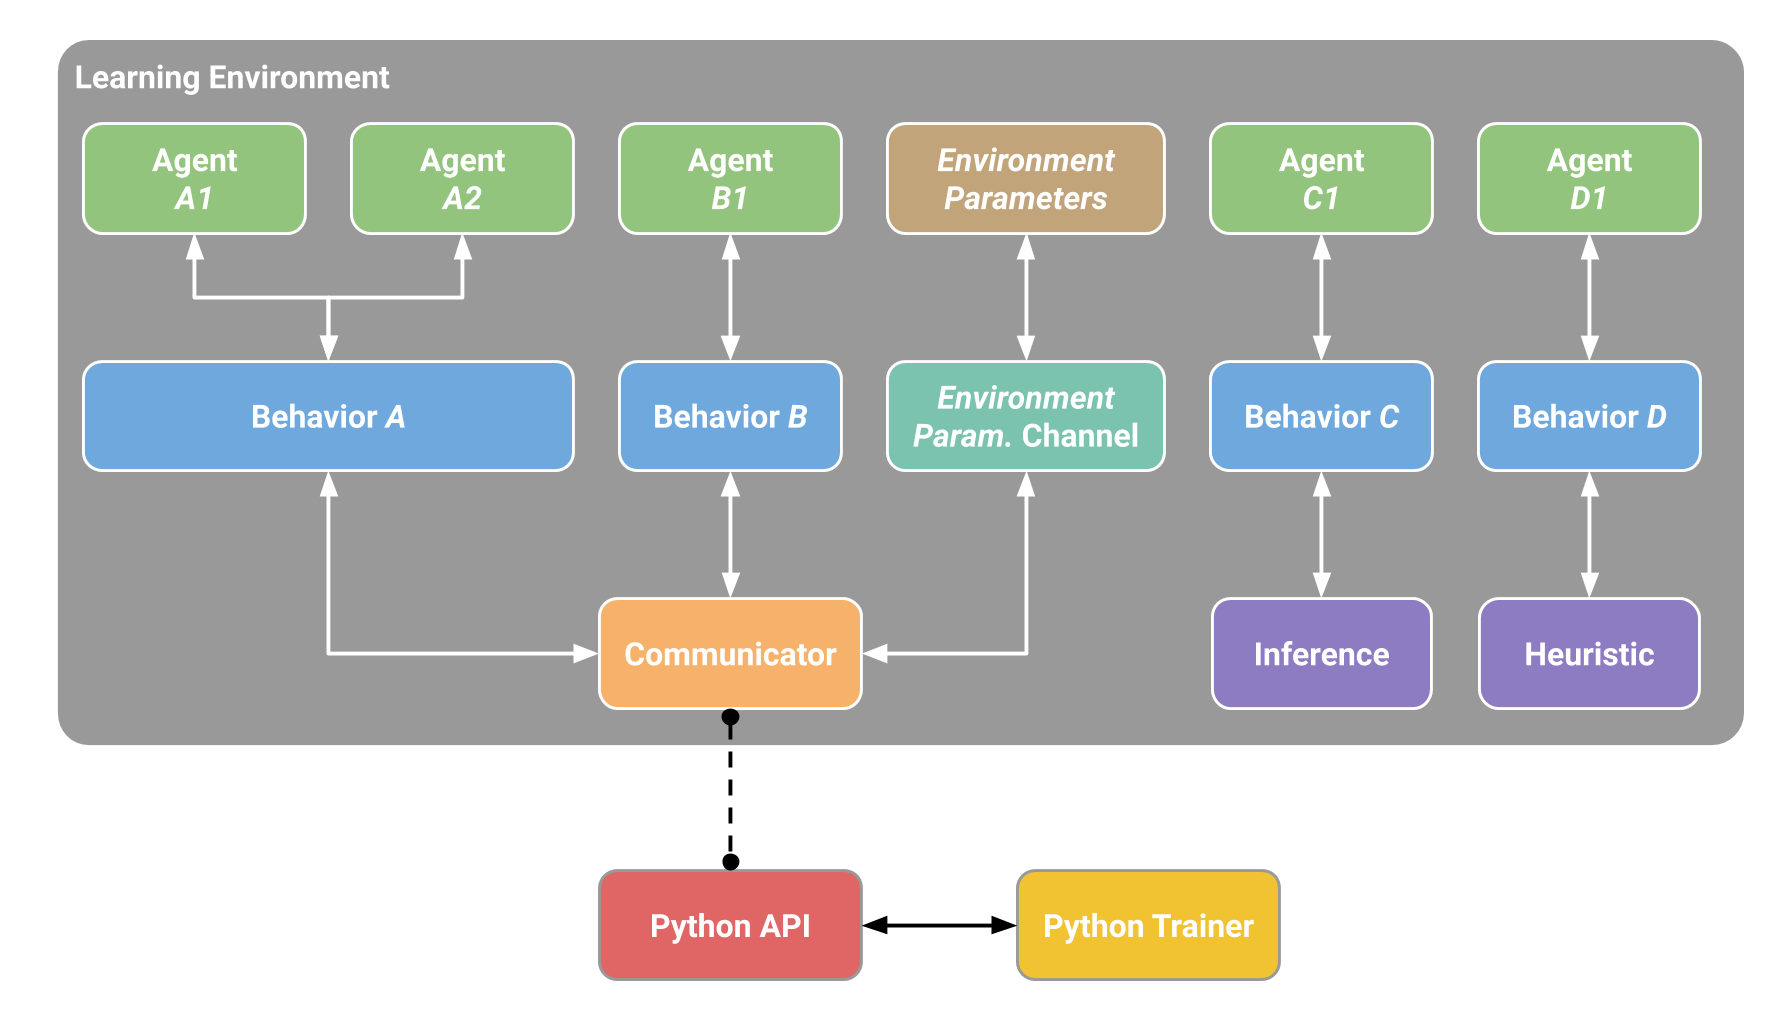
\includegraphics[width=1\textwidth]{image/learning_environment_full.png}
    \caption{Kiến trúc tổng thể của Unity ML-Agents Toolkit}
    \label{fig:mlagents_architecture}
\end{figure}

\subsubsection{Cơ chế Vật lý và Tính xác định trong Unity}
\indent Một khía cạnh cốt lõi khi sử dụng Unity cho học tăng cường là sự đồng bộ giữa hệ thống vật lý và quá trình ra quyết định. Trong Unity, các khung hình đồ họa được kết xuất qua hàm \texttt{Update()} với tần số biến thiên phụ thuộc vào hiệu năng máy tính (FPS). Tuy nhiên, nếu Agent cũng đưa ra quyết định hoặc tính toán va chạm theo tần số biến thiên này, môi trường sẽ trở nên không xác định (non-deterministic): cùng một chuỗi hành động có thể dẫn đến các kết quả vật lý khác nhau trong những lần chạy khác nhau.

\indent Để giải quyết vấn đề này, ML-Agents đồng bộ hóa toàn bộ quy trình RL vào hàm \texttt{FixedUpdate()}. Đây là chu kỳ cập nhật vật lý có tần số cố định (mặc định là $0.02$ giây mỗi bước, tương đương $50$ lần/giây). Hệ thống vật lý PhysX của Unity sẽ tính toán động lực học, cập nhật tọa độ của các \texttt{Rigidbody} và xử lý va chạm (\texttt{Collider}) hoàn toàn dựa trên các bước thời gian cố định này. Kết quả là, nếu cung cấp cùng một seed ngẫu nhiên ban đầu, môi trường Unity hoạt động như một hệ thống xác định: cùng một chuỗi hành động luôn cho ra cùng một quỹ đạo. Không có tính chất này thì mọi so sánh giữa hai lần chạy đều mất căn cứ.

\subsubsection{Hệ thống Cảm biến và Tiền xử lý quan sát}
\indent Để Agent hiểu được thế giới 3D phức tạp, ML-Agents cung cấp các thành phần Cảm biến nhằm tự động thu thập và chuyển đổi thông tin không gian thành các vector số thực (Input Layer). Có ba loại cảm biến phổ biến:
\begin{itemize}
    \item \textbf{Cảm biến tia (Ray Perception Sensor 3D)}: Bắn ra các tia raycast xung quanh Agent theo một góc quét nhất định. Khi tia chạm vào vật thể có nhãn (\texttt{Tags}) tương ứng, nó sẽ ghi nhận một vector one-hot đại diện cho loại vật thể và một giá trị vô hướng chuẩn hóa $[0, 1]$ biểu diễn khoảng cách. Đây là loại cảm biến đặc biệt hiệu quả và nhẹ về mặt tính toán cho các bài toán điều hướng, được áp dụng chủ đạo trong đề tài này.
    \item \textbf{Grid Sensor}: Chiếu một lưới 2D lên không gian và đếm số lượng vật thể rơi vào từng ô. Phù hợp cho các bài toán cần cái nhìn toàn cảnh như cờ bàn.
    \item \textbf{Camera Sensor}: Sử dụng trực tiếp dữ liệu pixel RGB từ camera, buộc mô hình phải dùng đến mạng tích chập (CNN). Dù cung cấp thông tin toàn diện, nó đòi hỏi chi phí tính toán rất lớn và thường hội tụ chậm hơn nhiều so với cảm biến tia.
\end{itemize}

\subsubsection{Cơ chế Hành vi và Gom nhóm quyết định}
\indent Một module quan trọng gắn trên mỗi Agent là \texttt{BehaviorParameters}, nơi định nghĩa kích thước không gian quan sát và không gian hành động. Tại đây, ML-Agents cung cấp cơ chế Action Masking (Mặt nạ hành động) để chặn các hành động không hợp lệ. Ví dụ, nếu Agent đang đứng sát tường, hệ thống có thể ``đeo mặt nạ'' loại bỏ hành động tiến lên, ép xác suất chọn hành động đó về 0. Điều này giúp thu hẹp không gian tìm kiếm, giúp mô hình hội tụ nhanh hơn thay vì phải tự học cách đâm đầu vào tường và bị phạt.

\indent Ngoài ra, thành phần \texttt{DecisionRequester} cho phép gom nhóm các bước mô phỏng (Decision Period). Thay vì đưa ra một quyết định mới ở mỗi bước \texttt{FixedUpdate} ($0.02$s), Agent có thể duy trì hành động cũ trong $5$ bước liên tiếp (Decision Period = $5$). Việc này giúp Agent có đủ thời gian hoàn thành một quỹ đạo vật lý trước khi quyết định tiếp, đồng thời giảm thiểu số lần gọi mạng nơ-ron lên nhiều lần, tối ưu hóa đáng kể tốc độ huấn luyện. ML-Agents cũng hỗ trợ Heuristic Policy, cho phép người dùng trực tiếp điều khiển Agent bằng bàn phím để gỡ lỗi và trải nghiệm độ khó của môi trường trước khi khởi động AI.

\subsubsection{Quy trình huấn luyện Agent}
\indent Quy trình huấn luyện một agent trong ML-Agents diễn ra theo vòng lặp lặp lại
liên tục cho đến khi đạt số bước tối đa hoặc người dùng dừng thủ công. Tại mỗi bước
thời gian, Unity thu thập quan sát từ tất cả các agent đang hoạt động trong scene,
gửi dữ liệu sang Python backend thông qua giao thức gRPC. Python trainer xử lý quan
sát, suy luận hành động từ policy hiện tại (hoặc lấy mẫu ngẫu nhiên trong giai đoạn
khởi động) và trả hành động về Unity. Unity thực thi hành động, cập nhật trạng thái
vật lý, tính toán phần thưởng và gửi kết quả trở lại Python để tích lũy vào buffer.

\indent Sau khi buffer tích lũy đủ một batch dữ liệu với kích thước do tham số
\texttt{buffer\_size} quy định, trainer tiến hành cập nhật tham số của mạng nơ-ron.
Đối với PPO, mỗi lần cập nhật gồm nhiều epoch chạy trên cùng một batch với hàm mục
tiêu clipped surrogate như đã trình bày tại Mục~\ref{sub:ppo}. Khi cập nhật hoàn tất,
buffer được xóa để mở đầu một chu kỳ thu thập dữ liệu mới, đồng thời các chỉ số huấn
luyện như cumulative reward, episode length và policy loss được ghi lại liên tục và
có thể theo dõi theo thời gian thực qua TensorBoard.

\indent Tệp cấu hình YAML kiểm soát toàn bộ quá trình huấn luyện. Tệp này định nghĩa
loại trainer (\texttt{trainer\_type}), các siêu
tham số huấn luyện (\texttt{hyperparameters}), kiến trúc mạng nơ-ron
(\texttt{network\_settings}), cấu hình tín hiệu phần thưởng (\texttt{reward\_signals})
và số bước huấn luyện tối đa (\texttt{max\_steps}). Mỗi behavior trong scene tương
ứng với một khối cấu hình riêng, cho phép huấn luyện đồng thời nhiều loại agent với
các thiết lập khác nhau trong cùng một session. Cấu hình chi tiết cho từng thuật toán
được trình bày trong các Phụ lục A đến D.

\subsubsection{Hỗ trợ thuật toán và giới hạn tích hợp sẵn}
\label{sub:mllimits}
\indent Unity ML-Agents phiên bản 4.0.2 tích hợp sẵn đúng ba trainer: \texttt{ppo} cho
bài toán đơn tác nhân và đối kháng, \texttt{poca} (MA-POCA) cho bài toán hợp tác đa tác
nhân, và \texttt{sac} như lựa chọn off-policy duy nhất. Kèm theo đó là các tín hiệu phần
thưởng nội tại như curiosity và RND để hỗ trợ khám phá trong môi trường phần thưởng
thưa. Người dùng lựa chọn thuật toán và cấu hình siêu tham số hoàn toàn thông qua tệp
YAML mà không cần thay đổi mã nguồn C\# của môi trường.

\indent Giới hạn đầu tiên nằm ngay ở danh sách đó: hai trong năm thuật toán mà đề tài
cần so sánh, MAPPO và DQN, không có mặt. Vì vậy chúng được bổ sung vào ML-Agents dưới
dạng trainer mở rộng, tức là các lớp trainer viết thêm rồi đăng ký vào cơ chế tra cứu
theo tên \texttt{trainer\_type}, nhờ đó dùng chung toàn bộ hạ tầng thu thập quỹ đạo,
ghi nhật ký TensorBoard và xuất mô hình ONNX với ba trainer có sẵn. Cách làm này giữ
cho năm thuật toán chạy trên cùng một đường ống đo đạc, điều kiện cần để mọi so sánh ở
Chương~\ref{ch:results} có ý nghĩa. Chi tiết được trình bày trong Mục~\ref{sub:custom}.

\indent Giới hạn thứ hai liên quan tới cơ chế tự chơi của môi trường đối kháng. Cơ chế
này được ML-Agents thiết kế quanh giả định chính sách là ngẫu nhiên và được cập nhật
theo lô on-policy; trên thực tế, PPO, MA-POCA, MAPPO và SAC đều ghép được với tự chơi
và đều sinh ra chỉ số ELO. Riêng DQN thì không: bộ điều phối đối kháng phát sinh lỗi
tra cứu chính sách ngay khi khởi tạo, nên lần chạy DQN trên Football Table buộc phải
tắt tự chơi và vì thế không có ELO để đối chiếu.

\indent Giới hạn còn lại liên quan tới phần thưởng nhóm. Cơ chế group reward được thiết
kế tối ưu cho POCA; khi áp dụng cho PPO, SAC hoặc DQN, phần thưởng nhóm buộc phải được
phân bổ thủ công về từng agent, làm suy giảm khả năng gán công lao. Ngoài ra, các
trainer tích hợp sẵn không cho phép người dùng dễ dàng can thiệp sâu vào vòng lặp huấn
luyện, chẳng hạn tùy biến hàm mất mát hay lịch trình cập nhật. Với những trường hợp cần
mức kiểm soát đó, thư viện \texttt{mlagents\_envs} cung cấp Python Low-Level API cho
phép điều khiển trực tiếp môi trường Unity như một môi trường kiểu Gym, từ đó kết nối
với các thư viện RL bên ngoài như Stable-Baselines3 \cite{raffin2021stable}.
